%##Capítulo 5. GeoDengue
\chapter{GeoDengue}
%* Introducción
A finales de los años 90, la información geográfica era mayoritariamente tratada en
supercomputadores, usada casi siempre para mantener registros internos de administraciones y el
software que se utilizaba para su manejo era stand-alone\citep{vgomesAegis2001}. Sin embargo, con
la aparición de internet, la demanda de acceso a la información ha crecido considerablemente
obligando a los sistemas de información geográfica a modificar su paradigma para ofrecer
información de forma distribuida.

Las autoridades sanitarias, en sus tareas de vigilancia en Salud Publica, tienen en los GIS una
herramienta fundamental para conocer como se extiende una enfermedad, estudiar su posible relacion
con un potencial foco de riesgo, o localizar un brote epidemico\citep{vgomesAegis2001}. En esta sección presentamos a GeoDengue una herramienta para identificación de focos de dengue
en un sistema de información georeferenciada.

%
El modelo solución para este problema se constituye de 4 partes fundamentales:

\begin{enumerate}[style=multiline,leftmargin=1.5cm]
    \item Establecimiento de puntos de control. Como primer paso es necesario fabricar los dispositivos de
     ovipostura (puntos de control, muestras) y distribuirlos en la zona o región que se desea analizazr. En el
     capítulo 5 se describe la estratégia implementada como mejor opción para la distribución de puntos de control.
     Además en el Anexo A se describe con detallada precisión la fabricación de los dispositivos de control;
     materiales, procedimiento, costos y recursos humanos necesarios
    
    \item Conteo. Una vez depositado el conjunto de muestras es necesario hacer un seguimiento para realizar el conteo de larvas que habitan en el dispositivo de control. Este conteo puede llevarse a cabo a los 7 días luego de que el dispositivo de ovipostura fue depositado. Es importante resaltar que un número mayor a 7 días podría significar que potenciales mosquitos hayan podido escapar del dispositivo de control por eso es necesario realizar el conteo antes de los 7 días o al séptimo día inclusive y luego vaciar el recipiente para volver a utilizarlo. 
    
    \item Procesamiento. El paso 3 y 4 constituyen básicamente el registro, procesamiento y análisis de los datos obtenidos de los conteos realizados. Ej: De un conjunto $D$ de 150 muestras, debemos tener 150 valores $z_{i}$ que representen los valores de la cantidad de larvas encontradas en cada dispositivo $d_{i}$. Al conjunto de valores $z_{i}$ se aplica un algoritmo de interpolación espacial que se encarga de generar una matriz de valores a partir de los datos de entrada. Este conjunto de valores contenidos en la matriz es utilizado para generar un mapa térmico que representa la propagación y distribución de las larvas en el contexto geoespacial.

    \item Análisis. El potencial analítico que provee la información generada es amplio y diverso. La primera alternativa de análisis y la más intuitiva es la identificación de los focos de la enfermedad. Además de ser el objetivo principal de la solución propuesta es una de las alternativas de mayor importancia ya que la identificación de focos de la enfermedad permite :
    \begin{itemize}
        \item Visualizar el estado actual y la distribución poblacional del mosquito \textit{Aedes Aegipty}.
        \item Realizar planes preventivos sobre zonas o regiones más afectadas.
        \item Implementar estrategias de fumigación y limpieza según zonas más afectadas.
        \item Otros.
    \end{itemize}
\end{enumerate}

\section{Descripción funcional}
GeoDengue es un sistema de información geográfico-sanitaria basado en una arquitectura cliente
servidor. Esta se presenta efectiva y concretamente todos los requerimientos que describen como el
software debe comportarse para cumplir con sus finalidades y objetivos. La aplicación se encuentra
dividida en sub módulos para, la gestión de datos de entrada, el simulador del proceso evolutivo y
presentación de los datos.


\subsection{Gestión de datos de entrada}
%Muestras
El sistema requiere principalmente de 2 datos de entrada, los putnos de control y los datos
climatólogicos correspondientes a el periodo de tiempo para la simulación

El área de estudio se encuentra determinada por una muestra, que representan a un conjunto de
puntos de control georeferenciados en una zona determinada. Los puntos de control que pertenecen a
una muestra deben ser establecidos en un mismo instante, siendo así la fecha de instalación y
fecha de recolección, de los puntos de control de la muestra, iguales.


Los puntos de control, como resultado de la medición realizada, permiten obtener la densidad de
larvas asociada con la información geográfica.
%Gestión de puntos de control
\subsection{Simulador del proceso evolutivo}

La simulación del prorceso evolutivo del mosquito del aedes aegypti requiere principalmente los
puntos de control pertenecientes el área de estudio y los datos climatológiocs del correspondientes
a dicha área. El proceso evolutivo consta de varios pasos, el desarrollo, la mortalidad,
la ovipostura y dispersión de los individuos de la población.

El proceso inicia al procesar los puntos de control pertenecientes a la muestra utilizada para el
estudio. La población inicial se encuentra compuestas por las larvas observadas en la muestra
utilizada para el estudio. Una vez generada la población inicial se obtienen los datos
climatológicos correspondientes, desde la fecha de recolección de los puntos de contro, hasta un
periodo máximo de 30 días. Se establece un periodo máximo debido los serivicios de predicción del
clima utilizados establecen dicho tope.

\begin{algorithm}
\caption{Simulación del proceso evolutivo}
\label{alg:simulador-evolutivo}
\begin{algorithmic}[1]
    \REQUIRE $\vec{k}\neq \emptyset \land \vec{m} \neq \emptyset$
    \ENSURE $\vec{m'}$
    \FORALL{$k{i} \in \vec{k}$ }
        \STATE $\vec{huevos} \Leftarrow \emptyset$
        \FORALL{$m{j} \in \vec{m}$}
            \STATE $desarrollar(m_{j}, k_{i})$
            \IF{$regular(m_{j}, k_{i})$}
                \STATE \COMMENT{Se elimina $m_{j}$ si es un candidato.}
                \STATE $m_{j} \Leftarrow \varnothing $
            \ELSIF{$esta\_maduro(m_{j}, k_{i})$}
                \STATE $ cambiar\_estado(m_{j}) $
            \ELSIF{$se\_reproduce(m_{j})$}
                \STATE $\vec{huevos} \Leftarrow \vec{huevos} + oviponer(m_{j})$
            \ENDIF
        \ENDFOR

        \IF{$\vec{huevos} \neq \emptyset$}
            \STATE \COMMENT{Si ovipone se extiende la población}
            \STATE $\vec{m} \Leftarrow  \vec{m} + \vec{huevos}$
        \ENDIF
    \ENDFOR
    \RETURN $\vec{m}$
\end{algorithmic}
\end{algorithm}

El \algref{alg:simulador-evolutivo}, describe al simulador como un proceso iterativo cuyo objetivo
es simular los efectos de cada $k_{i}$ para cada individuo $m_{j}$ que pertenezca a la población.


\begin{algorithm}
\caption{$desarrollar(m_{j}, k_{i})$}
\label{alg:desarrollo}
\begin{algorithmic}[1]
    \REQUIRE $ k{i} \neq \varnothing \land m{j} \neq \varnothing$
    \ENSURE $m'_{j}$
            \STATE $d_{j} \Leftarrow d_{j -1} + R(k_{i})$
            \IF{$m_{j}\ es\ adulto$}
            \STATE $volar(m_{j}, k_{i})$
            \ENDIF
    \RETURN $m_{j}$
\end{algorithmic}
\end{algorithm}

%* Diseño y Arquitectura
\section{Diseño y Arquitectura}
GeoDengue está basada en una arquitectura, de tres capas, cliente-servidor, en el que las tareas
se reparten entre los proveedores de recursos o servicios, denominados servidores, y los
demandantes, llamados clientes. La primera capa, la de presentación, es la que se encarga de
interactuar con el usuario final, la segunda capa es la de negocios, esta se encarga de procesar
las solicitudes realizadas por la capa de presentación y definir las reglas que deben aplicase en
para cada solicitud. Por último, se encuentra la capa de datos, donde se almacenan los datos,
porcesan las peticiones de la capa de negocios para persistir o recuperar información.

\begin{figure}
\centering
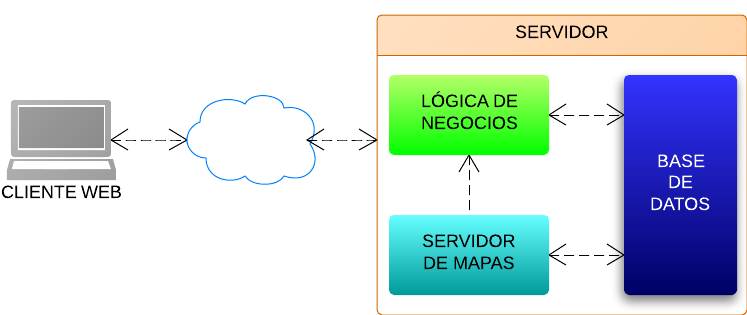
\includegraphics[width=0.9\textwidth]{capitulo-5/graphics/arquitectura-completa.png}
\caption{\label{fig:arquitectura-completa}Arquitectura de interacción de componentes de GeoDengue.}
\end{figure}

Se optó por un enfoque web debido a la practicidad de estas aplicaciones, el usuario final solo
debe contar con un navegador web. Estas deberían funcionar igual independientemente de la versión
del sistema operativo instalado en el cliente. Las aplicaciones web son catalogadas como
aplicaciones de bajo consumo, debido a que la mayor parte de la aplicación no se encuentra en
nuestro ordenador, y muchas de las tareas de procesamiento que realiza el software no consumen
recursos nuestros porque se realizan en el servidor.

La capa de presentación se encuentra diseñada como un Single Page Application o SPA (en español
Aplicación de una sola página). Un SPA es una aplicación que se ejecuta en una única página, donde
la navegación se realiza mediante cargas parciales, sin recargar el sitio completamente. La
comunicación con el servidor se realiza mendiante peticiones Ajax, para ello se cuenta con una
arquitectura basada en servicios REST.


%* Tecnologías y herramientas utilizadas
\section{Tecnologías y herramientas utilizadas}

Una vez analizadas las funcionalidades del sistema, se tomo la decisión de implementar la herramienta
como aplicación web por su orientación a múltiples usuarios y a la localización geográfica de contenidos,
es decir, que su objetivo está orientada a un uso online cuyo contenido depende de las aportaciones de
diferentes usuarios. Así también se evita un problema de las aplicaciones standalone, que obligan a que
se tenga que instalar el software en los equipos cliente, con la consiguiente dificultad de acceso a la
herramienta. En el caso de las aplicaciones web tan solo se necesita un navegador web para su acceso,
aunque en este caso ha de ser lo suficientemente reciente para soportar las tecnologías que se emplean.

Las tecnologías utilizadas en el desarrollo de la aplicación fueron <TODO>

para el procesamiento digital de imágenes se utilizó el paquete <TODO> de python

Como servidor de aplicaciones web se utilizó apache, con respecto al almacenamiento de datos, 
se decidió usar el sistema gestor de bases de datos PostgreSQL , por ser de uso libre y por 
cuestiones referentes a los datos geográficos ya que dispone de la extensión PostGIS para su manejo.


En lo referente a las tecnologías GIS empleadas, puesto que la aplicación ofrecerá la posibilidad 
de visualizar, consultar y modificar información geográfica, los estándares de OGC con los que trabaja, directa o indirectamente, son GML, WFS, WMS, SLD,
Filter Encoding y documentos de contexto de mapas (Web Map Context Documents, WMC).

El servidor de información geográfica Geoserver. 


El Cliente de información geográfica Mapbuilder. Genera mapas y realiza peticiones, 
interactuando con el servidor GIS a través de los estándares OGC. Es una Librería que 
implementa un entorno para crear el contenido de una página web mediante el procesamiento 
de documentos XML usando la tecnología AJAX.


\subsection{GeoServer}
El proyecto GeoServer en una aplicación Java que integra la versión 1.0 de WFS,
1.1.1 de WMS y 1.0 de WCS para poder publicar información bien directamente permi-
tiendo su manipulación, bien en forma de imágenes o mapas. Geoserver tiene en cuenta
cuatro metas principales en el ámbito de desarrollo, ordenadas por importancia:
Cumplimiento de los estándares: El proyecto GeoServer intenta promover la estandarización, 
y soportar tantos estándares como sea posible, para permitir a todos compartir su información 
geoespacial rápidamente y de una forma interoperable, disminuyendo así las barreras entre 
proveedores de información geográfica.
Soporte para diferentes formatos información: Para hacer un producto útil, GeoServer intenta 
traducir todos los formatos de datos de información geográfica en uno solo. Sin embargo, 
el soporte para varios formatos de datos es una de las prioridades. Actualmente soporta 
eficientemente almacenamiento en los formatos shapefile, PostGIS, DB2, Oracle, ArcSDE y, 
además ofrece servicio para soportes en prueba como MySQL, Vector Product Format Library 
(VPF), Web Feature Server (WFS) y MapInfo. Y en cuanto a los formatos de salida que Geoserver
puede generar como respuesta a peticiones WFS-T y WMS se encuentran, entre
otros:
• JPEG: Joint Photographic Experts Group, algoritmo de compresión de imágenes con pérdida 
de información.
• PNG: Portable Network Graphics, algoritmo de compresión de imágenes sin
pérdida de información.
• SVG: Scaleable Vector Graphics, lenguaje para describir gráficos vectoriales
bidimensionales.
• GML: Geography Markup Language.
• PDF: Portable Document Format, formato de almacenamiento de documentos, desarrollado 
por la empresa Adobe Systems.
• shapefiles: formato propietario abierto de datos espaciales desarrollado por la compañía ESRI,
originalmente creado para su producto ArcView GIS, pero actualmente se ha convertido en formato estándar
de facto por la importancia que los productos ESRI tienen en el mercado SIG. Un Shapefile es un formato
vectorial de almacenamiento digital donde se guarda la localización de los elementos geográficos y los
atributos asociados a ellos. El formato carece de capacidad para almacenar información topológica.

• KML/KMZ: Keyhole Markup Language, lenguaje de marcado basado en XML para representar datos geográficos
en tres dimensiones, desarrollado para ser manejado con Google Earth. 

Fácil de usar: Fácil de instalar, configurar y ejecutar para organizaciones con pocos recursos técnicos. Orientado para organizaciones con experiencia técnica mínima.

Eficiencia: El procesado de información geográfica normalmente requiere muchas cargas computacionales y
de ancho de banda, GeoServer intenta minimizar ambas. Desde el punto de vista del usuario, GeoServer es
una herramienta necesaria para mostrar mapas en las paginas web, donde el usuario puede hacer zoom,
cambiar la vista y hacer operaciones soportadas por los especificaciones WMS y WFS de OGC.

Es usado en conjunto con clientes como MapBuilder, con el objetivo de conectar facil y54
2. Tecnologías y software GIS eficientement bases de datos geográficas con clientes GIS. 
El uso de estándares permite combinar la información del GeoServer fácilmente con otra información 
geográfica

%   * Lenguajes de programación tanto para el backend y el frontend
%   * Servidor de aplicaciones (apache)
%   * Bases de datos
%   * Servidor de mapas (geoserver)

% * Herramienta para la identificación de focos de dengue en un sistema de información gerefernciada.

%    * muestras
%    * puntos de control y colonias
%    * Conteo de larvas mediante procesamiento digital de imágenes
%\section{Conteo de larvas mediante procesamiento digital de imágenes}
Llamamos procesamiento digital de imágenes (PDI) al conjunto de técnicas de para alterar o extraer
información de imágenes digitales. Existe una inmensa cantidad de contenido de imágenes digitales 
(cámaras de seguridad, fotografías personales, contenido web de blogs, noticias y eventos, etc.). 
De dicha cantidad de datos en formato de imágenes digitales existe cada vez más mayor necesidad
de procesarlos para generar el contenido deseado. 
Una aplicación práctica sería aplicar un filtro visual a una imagen. Existen distintos tipos de 
filtros gráficos como vintage, por puntos, tipo antigua, poster y otros que mediante un algoritmo 
PDI puede ser aplicados a una imagen. Como ejemplo; tomar una fotografía actual y aplicar un filtro de foto antigua. Esta aplicación práctica representa el procesamiento para la alteración de imágenes.

La aplicación práctica menos más compleja es el procesamiento de imágenes para la extracción de 
información. Es más sencillo rotar una imagen que realizar un análisis de cuantas personas se 
encuentran en dicha imagen. Análogo al proceso de alterar imágenes existen varias técnicas para la
extracción de información a partir de objetos visuales digitales. Una aplicación práctica sería
identificar el número de chapa de un vehículo al cual se le tomó una fotografía al infringir una 
ley de tránsito.

Para este trabajo utilizamos PDI para resolver y automatizar un proceso fundamental para nuestro
sistema; Realizar el conteo de larvas en un recipiente de ovipostura. El conteo de larvas se realiza 
de la siguiente manera:

\begin{enumerate}
    \item Se toma una (o más) fotografía(s) al dispositivo de ovipostura del cual se quiere conocer el 
    número de larvas.
    \item Se guarda la fotografía en el servidor para ser analizado.
    \item Un algoritmo que utiliza técnicas de PDI analiza la imagen y obtiene la cantidad de larvas
    contenidas en la misma.
\end{enumerate}

En el modelo propuesto utilizamos el algoritmo de Otsu explicado en la siguiente sección para la
segmentación mediante umbrales y un algoritmo de no aproximación para la identificación de contornos
para las imágenes.

\subsection{Método Otsu}
Dentro de el área de PDI (procesamiento digital de imágenes) existen diferentes métodos de análisis
de imágenes con distintas características y para distintos fines. Ya sea que necesitemos realizar
reconocimiento de rostros, formas o figuras, o realizar cualquier tipo de procesamiento con las 
imágenes existe un método o un conjunto de procesos que cumplen la función que necesitamos.

Uno de los métodos dentro del campo de PDI es el método de Otsu. Este es un método de segmentación por
umbralización. La umbralización es el proceso de establecer umbrales (valores máximos y mínimos) que se
aplican al análisis de una imagen. Cada píxel es discriminado según los valores umbrales para determinar
a qué grupo pertenece. Un ejemplo práctico conceptual sería pasar una imagen en colores a una misma
imagen en blanco y negro. Para ello necesitamos definir un umbral, un valor que nos determine si 1 píxel
analizado pertenece al grupo de los ”blancos” o de los ”negros” dependiedo de su color actual. Sí el
color del píxel es un rojo intenso entonces lo incluimos en el conjunto de los ”negros” y si el color es
más bien claro, como blanco o gris claro entonces lo agregamos al grupo de los ”blancos”.

Este método lo utilizamos en nuestro trabajo para, a partir de una fotografía de las larvas, hacer un
traspaso a una imagen a escala de grises, la cual puede ser analizada por un algoritmo de conteo y así
realizar el conteo de las larvas.

En primer lugar definimos 2 conjuntos. El conjunto de objetos dentro de la imagen(e: las larvas) y el
fondo(ej: el recipiente con el agua que contiene las larvas). Luego definimos el umbral ”T” que
determina si un píxel pertenece a un grupo u otro según su nivel de gris ”g”. La función ”f” retorna 1 
o 0 por cada píxel (par de coordenadas ”x” e ”y”).

\begin{equation}
f(x, y) =\left\{
  \begin{array}{l l}
    1 & \quad g > T\\
    0 & \quad g \leq T
  \end{array} \right.
\end{equation}

Como se observa en la ecuación se analiza simplemente el nivel de gris en cada píxel y se determina si
forma parte de un objeto de estudio o si forma parte del fondo.

%    * simulación del porceso evolutivo
%\subsection{Análisis de datos}
El gran potencial analítico de la información generada por los puntos de control y el simulador
del proceso evolutivo, permiten la implementación diferentes tipos de análisis estadísticos y
geográficos. De forma básica se han implementado la cartografía del vector, la identificación de
focos y el análisis del ciclo de vida del vector.

\subsubsection{Cartografía del vector}
La cartografía del vector, es empleada para representar geográficamente la distribución espacial
del vector \citep{vgomesAegis2001}. Esta es obtenida a partir de los puntos de control establecidos
previamente, donde, cada uno se encuentra asociado a con nivel de criticidad.

\subsubsection{Identificación de focos de infestación}
\label{sec:cap5-identificacion-focos}
El proceso de identificación de focos de infestación fue previamente presentado en la
\secref{sec:cap4-identificacion-focos}, es el encargado de transformar la información obtenida de
los puntos de control distribuidos geográficamente, mediante métodos de interpolación, en mapas
donde se puede apreciar los niveles de riesgo correspondientes.

La selección del método de interpolación se realizó teniendo en cuenta el factor humano en la
distribución de los puntos de control. En \cite{villatoro2007comparacion} se realiza una
comparación de los interpoladores IDW y Kriging, donde los autores señalan que el método Kriging
fue más preciso y eficiente que el IDW, aunque la diferencia entre ambos métodos no fue muy amplia.
Sin embargo, cuando el distanciamiento, es muy grande, los variogramas no son posibles de obtener,
entonces el Kriging deja de ser una opción y comparativamente el IDW se perfila como el mejor
\cite{villatoro2007comparacion}. El método seleccionado finalmente fue el IDW, debido que la
distribución del los puntos de control no será perfecta, inclusive, en algunas localidades la
distribución no será de forma uniforme.

\subsubsection{Análisis del ciclo de vida del vector}
El análisis del ciclo de vida del vector consiste en procesar la información generada durante el
proceso evolutivo para determinar :

\begin{itemize}
    \item \textit{Duración promedio del ciclo de vida}, determina la duración en días de cada etapa de desarrollo del vector, con esto podemos determinar que tan rápido puede desarrollarse al población.

    \item \textit{Tasa de mortalidad diaria} indica el porcentaje de reducción diario de la población.

    \item \textit{Duración del ciclo gonotrófico}, calcula la duración promedio, en días, del ciclo gonotrófico de las hembras adultas nulíparas y paridas.

    \item \textit{Rango de dispersión}, indica el radio promedio de vuelo, en metros, del adulto tomando como origen el lugar donde emergió.

\end{itemize}

%    * reportes estadisticos implementados
%       + Crecimiento de la población
%       + Tasas de desarrollo
%       + %Mortalidad
%       + Dispersión

%    * interpolación de puntos de control
%    * historial de enventos (superposicion de layers)


%* Estructuras de datos y algoritmos utilizados
%\section{Algoritmos y estructuras de datos utilizadas}


